\documentclass[11pt]{beamer}
\usetheme{Madrid}
\usecolortheme{default}

\usepackage{fontspec}
\usepackage{listings}
\usepackage{xcolor}
\usepackage{tikz}
\usetikzlibrary{shapes.symbols, shapes.arrows, positioning}
\setmainfont{Arial}         % font co san tren Windows, ho tro tieng Viet
\setmonofont{Consolas}      % font code, ho tro dau tieng Viet

\definecolor{codebg}{RGB}{245,245,245}
% Mau cho so do cac kieu du lieu
\definecolor{dtA}{RGB}{ 77,199,190}
\definecolor{dtB}{RGB}{ 26,180,168}
\definecolor{dtC}{RGB}{ 58,199,235}
\definecolor{dtD}{RGB}{ 42,140,206}
\definecolor{dtE}{RGB}{ 22, 71,124}
\lstset{
  language=Python,
  backgroundcolor=\color{codebg},
  basicstyle=\ttfamily\small,
  keywordstyle=\color{blue}\bfseries,
  commentstyle=\color{gray}\itshape,
  stringstyle=\color{orange},
  showstringspaces=false,
  breaklines=true,
  extendedchars=true,
  inputencoding=utf8,
  frame=single,
  numbers=left,
  numberstyle=\tiny\color{gray},
}

\title{Python cơ bản}
\author{Trình bày: Võ Luyện}
\date{}

\begin{document}

\frame{\titlepage}

\begin{frame}{Nội dung buổi học}
\tableofcontents
\end{frame}

\section{Python là gì?}

\begin{frame}{Python là gì?}
\begin{itemize}
  \item Python là ngôn ngữ lập trình bậc cao, cú pháp gần với ngôn ngữ tự nhiên, dễ đọc
  \item Ra đời năm 1991, hiện là một trong những ngôn ngữ được dùng nhiều nhất thế giới
  \item Là ngôn ngữ thông dịch (interpreter) — chạy trực tiếp từng dòng lệnh, không cần biên dịch phức tạp
  \item Có hệ sinh thái thư viện khổng lồ: xử lý dữ liệu, web, tự động hóa, và đặc biệt là \textbf{Trí tuệ nhân tạo / Machine Learning}
\end{itemize}
\end{frame}

\begin{frame}{Vì sao Python là lựa chọn số 1 cho AI?}
\begin{itemize}
  \item Cú pháp đơn giản $\to$ tập trung vào ý tưởng thuật toán thay vì vật lộn với ngôn ngữ
  \item Thư viện và framework phong phú:
  \begin{itemize}
    \item Trực quan hóa và xử lý dữ liệu: NumPy, Pandas và Seaborn
    \item Machine learning: Scikit-learn, XGBoost và LightGBM
    \item Deep learning: PyTorch, TensorFlow và Keras
  \end{itemize}
  \item Cộng đồng lớn, tài liệu phong phú, dễ tìm hỗ trợ khi gặp lỗi
  \item Hầu hết các cuộc thi và nghiên cứu AI hiện nay đều dùng Python làm ngôn ngữ chính
\end{itemize}
\end{frame}

% \section{Các cuộc thi AI cho học sinh THPT}

% \begin{frame}{Các cuộc thi AI dành cho học sinh THPT}
% \begin{itemize}
%   \item \textbf{IOAI (International Olympiad in AI)} — kỳ thi Olympic Quốc tế về Trí tuệ nhân tạo, gồm phần thi lý thuyết và thực hành ML/NLP/CV
%   \item \textbf{Olympic Tin học THPT / Tin học trẻ} — nền tảng thuật toán và lập trình cơ bản
%   \item \textbf{AI Hackathon dành cho học sinh} — các cuộc thi làm dự án AI theo nhóm, thời gian ngắn
%   \item \textbf{Kaggle Competitions (mức nhập môn)} — luyện tập xử lý dữ liệu thật, xây mô hình dự đoán
%   \item Tham gia các cuộc thi này giúp rèn kỹ năng lập trình, tư duy giải quyết vấn đề và làm quen với quy trình xây dựng mô hình AI thực tế
% \end{itemize}
% \end{frame}

\section{Các công cụ lập trình Python}

\begin{frame}{Các công cụ lập trình Python}
\begin{itemize}
  \item \textbf{IDLE} — trình soạn thảo đi kèm khi cài Python, đơn giản, phù hợp người mới bắt đầu
  \item \textbf{VS Code} — trình soạn thảo phổ biến, nhẹ, có extension hỗ trợ Python mạnh mẽ
  \item \textbf{PyCharm} — IDE chuyên dụng cho Python, nhiều công cụ debug và quản lý dự án
  \item \textbf{Jupyter Notebook} — chạy code theo từng ô (cell), phù hợp thử nghiệm, phân tích dữ liệu và AI
  \item \textbf{Google Colab} — Jupyter Notebook chạy trên trình duyệt, miễn phí, có sẵn GPU — không cần cài đặt máy tính
\end{itemize}
\end{frame}

\section{Cú pháp cơ bản của Python}

\begin{frame}[fragile]{Câu lệnh bắt đầu và kết thúc như thế nào?}
\begin{itemize}
  \item Mỗi câu lệnh Python nằm trên \textbf{một dòng}, kết thúc khi \textbf{xuống dòng}
  \item \textbf{Không} cần dấu chấm phẩy \texttt{;} ở cuối câu như C/C++/Java
  \item Không dùng dấu ngoặc nhọn \texttt{\{ \}} để gom nhóm lệnh
\end{itemize}
\begin{lstlisting}
x = 10          # one statement
y = 20          # another statement
print(x + y)    # a statement ends at the end of the line
\end{lstlisting}
\end{frame}

\begin{frame}[fragile]{Viết một câu lệnh dài trên nhiều dòng}
Khi câu lệnh quá dài, có thể ngắt dòng cho dễ đọc:
\begin{lstlisting}
# Way 1: use a backslash \
tong = 1 + 2 + 3 + \
       4 + 5 + 6

# Way 2: inside () [] {} lines are joined automatically
tong = (1 + 2 + 3 +
        4 + 5 + 6)

diem = [8.5, 7.0,
        9.5, 6.0]
\end{lstlisting}
\end{frame}

\begin{frame}[fragile]{Thụt lề (Indentation)}
\begin{itemize}
  \item Python dùng \textbf{thụt lề} để xác định khối lệnh (block), thay cho \texttt{\{ \}}
  \item Chuẩn: thụt vào \textbf{4 dấu cách} cho mỗi cấp
  \item Thụt lề sai $\to$ chương trình báo lỗi \texttt{IndentationError}
\end{itemize}
\begin{lstlisting}
if diem >= 5:
    print("Dat")        # inside the if block (indented 4 spaces)
    print("Chuc mung")  # same block
print("Ket thuc")       # NOT inside if (no indentation)
\end{lstlisting}
\end{frame}

\begin{frame}[fragile]{Dấu hai chấm (:) mở đầu một khối lệnh}
Dấu \texttt{:} báo hiệu "phía dưới là một khối lệnh, hãy thụt lề vào".
\begin{lstlisting}
if x > 0:           # colon here
    print("Duong")

for i in range(3):  # colon here
    print(i)

while x > 0:        # colon here
    x = x - 1

def chao(ten):      # colon here
    print("Xin chao", ten)
\end{lstlisting}
\end{frame}

\begin{frame}[fragile]{Comment — ghi chú trong code}
\begin{itemize}
  \item Comment là dòng \textbf{giải thích} cho người đọc, Python \textbf{bỏ qua} khi chạy
  \item Comment một dòng: bắt đầu bằng dấu \texttt{\#}
  \item Comment nhiều dòng: dùng ba dấu nháy \texttt{"""} hoặc \texttt{'''}
\end{itemize}
\begin{lstlisting}
# This is a single-line comment

x = 10  # inline comment, explains the variable x

"""
This is a multi-line comment.
It is often used to describe a program
or the purpose of a function.
"""
\end{lstlisting}
\end{frame}

\begin{frame}[fragile]{Quy tắc đặt tên biến}
\begin{itemize}
  \item Chỉ gồm chữ cái, chữ số và dấu gạch dưới \texttt{\_}
  \item \textbf{Không} bắt đầu bằng chữ số, \textbf{không} chứa dấu cách
  \item \textbf{Phân biệt} chữ hoa và chữ thường: \texttt{diem} $\neq$ \texttt{Diem}
  \item Không dùng từ khóa của Python (\texttt{if}, \texttt{for}, \texttt{class}, \texttt{print}...)
  \item Quy ước: dùng \texttt{snake\_case} — chữ thường, nối bằng gạch dưới
\end{itemize}
\begin{lstlisting}
diem_trung_binh = 8.5   # OK, easy to read
ten_hoc_sinh = "An"     # OK

2diem = 5     # WRONG: starts with a digit
diem tb = 5   # WRONG: contains a space
for = 10      # WRONG: 'for' is a keyword
\end{lstlisting}
\end{frame}

\begin{frame}[fragile]{Lỗi cú pháp thường gặp}
\begin{lstlisting}
# Missing colon
if x > 0
    print("Duong")        # SyntaxError

# Wrong indentation
if x > 0:
print("Duong")            # IndentationError

# Mixing tabs and spaces -> always use 4 spaces

# Missing closing parenthesis
print("Xin chao"          # SyntaxError
\end{lstlisting}
\end{frame}

\section{Biến và kiểu dữ liệu}

\begin{frame}[fragile]{Biến (Variables)}
\begin{itemize}
  \item Python không cần khai báo kiểu dữ liệu trước
  \item Gán giá trị bằng dấu \texttt{=}
\end{itemize}
\begin{lstlisting}
name = "An"
age = 17
height = 1.65
is_student = True
\end{lstlisting}
\end{frame}

\begin{frame}{Các kiểu dữ liệu trong Python}
\vspace{0.3cm}
\begin{center}
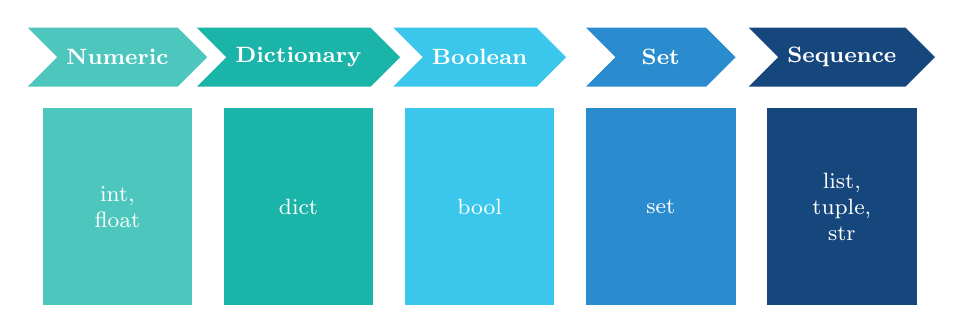
\begin{tikzpicture}[
  chev/.style={
    signal, signal to=east, signal from=west,
    minimum width=1.9cm, minimum height=0.75cm,
    text=white, font=\bfseries\footnotesize, align=center
  },
  box/.style={
    minimum width=1.9cm, minimum height=2.5cm,
    text=white, font=\footnotesize, align=center
  }
]
\node[chev, fill=dtA] (c1) at (0,0)   {Numeric};
\node[chev, fill=dtB] (c2) at (2.3,0) {Dictionary};
\node[chev, fill=dtC] (c3) at (4.6,0) {Boolean};
\node[chev, fill=dtD] (c4) at (6.9,0) {Set};
\node[chev, fill=dtE] (c5) at (9.2,0) {Sequence};

\node[box, fill=dtA] at (0,-1.9)   {int,\\ float};
\node[box, fill=dtB] at (2.3,-1.9) {dict};
\node[box, fill=dtC] at (4.6,-1.9) {bool};
\node[box, fill=dtD] at (6.9,-1.9) {set};
\node[box, fill=dtE] at (9.2,-1.9) {list,\\ tuple,\\ str};
\end{tikzpicture}
\end{center}
\end{frame}

\begin{frame}[fragile]{Nhóm Numeric — kiểu số}
\begin{itemize}
  \item \textbf{int}: số nguyên, không giới hạn độ lớn
  \item \textbf{float}: số thực (số thập phân)
\end{itemize}
\begin{lstlisting}
tuoi = 17           # int
chieu_cao = 1.65    # float

print(type(tuoi))       # <class 'int'>
print(type(chieu_cao))  # <class 'float'>
\end{lstlisting}
\end{frame}

\begin{frame}[fragile]{Boolean — kiểu logic}
\begin{itemize}
  \item Chỉ có \textbf{hai} giá trị: \texttt{True} và \texttt{False} (viết hoa chữ đầu)
  \item Là kết quả của mọi phép so sánh
  \item Bản chất là số: \texttt{True} = 1, \texttt{False} = 0
\end{itemize}
\begin{lstlisting}
la_hoc_sinh = True
da_dat = 7 >= 5     # True

print(True + True)  # 2
print(bool(0))      # False
print(bool(""))     # False (empty string)
print(bool("An"))   # True
\end{lstlisting}
\end{frame}

\begin{frame}[fragile]{Nhóm Sequence — dãy có thứ tự}
\begin{itemize}
  \item \textbf{str}: chuỗi ký tự — không thay đổi được (immutable)
  \item \textbf{list}: danh sách — \textbf{thay đổi được}, dùng \texttt{[ ]}
  \item \textbf{tuple}: giống list nhưng \textbf{không đổi được}, dùng \texttt{( )}
  \item Điểm chung: có \textbf{chỉ số} (index) bắt đầu từ 0
\end{itemize}
\begin{lstlisting}
ten = "Python"            # str
diem = [8.5, 7.0, 9.0]    # list
toa_do = (10, 20)         # tuple

print(ten[0])     # 'P'  - the first character
print(diem[1])    # 7.0
diem[1] = 8.0     # OK, a list is mutable
toa_do[0] = 5     # ERROR! a tuple is immutable
\end{lstlisting}
\end{frame}

\begin{frame}[fragile]{Set và Dictionary}
\begin{itemize}
  \item \textbf{set}: tập hợp, \textbf{không trùng lặp}, không có thứ tự — dùng \texttt{\{ \}}
  \item \textbf{dict}: từ điển, lưu theo cặp \textbf{khóa : giá trị} (key : value)
\end{itemize}
\begin{lstlisting}
mon_hoc = {"Toan", "Ly", "Toan"}
print(mon_hoc)    # {'Toan', 'Ly'} - duplicates removed

hoc_sinh = {"ten": "An", "tuoi": 17}
print(hoc_sinh["ten"])   # An
\end{lstlisting}
\end{frame}

\begin{frame}[fragile]{Ép kiểu dữ liệu (Type casting)}
Chuyển đổi giữa các kiểu bằng các hàm \texttt{int()}, \texttt{float()}, \texttt{str()}, \texttt{bool()}:
\begin{lstlisting}
s = "25"
n = int(s)          # 25   (str -> int)
f = float(s)        # 25.0 (str -> float)

x = 3.9
print(int(x))       # 3  (truncates, does NOT round)

tuoi = 17
print("Tuoi: " + str(tuoi))   # must cast to str to concatenate

int("abc")   # ERROR: ValueError
\end{lstlisting}
\end{frame}

\section{Toán tử trong Python}

\begin{frame}[fragile]{Toán tử số học (Arithmetic)}
\begin{center}
\begin{tabular}{|c|l|c|}
\hline
\textbf{Toán tử} & \textbf{Ý nghĩa} & \textbf{Ví dụ (a=10, b=3)} \\
\hline
\texttt{+}  & Cộng                  & \texttt{a + b} $\to$ 13 \\
\texttt{-}  & Trừ                   & \texttt{a - b} $\to$ 7 \\
\texttt{*}  & Nhân                  & \texttt{a * b} $\to$ 30 \\
\texttt{/}  & Chia (luôn ra float)  & \texttt{a / b} $\to$ 3.333 \\
\texttt{//} & Chia lấy phần nguyên  & \texttt{a // b} $\to$ 3 \\
\texttt{\%} & Chia lấy phần dư      & \texttt{a \% b} $\to$ 1 \\
\texttt{**} & Lũy thừa              & \texttt{a ** b} $\to$ 1000 \\
\hline
\end{tabular}
\end{center}
\vspace{0.2cm}
\small \texttt{\%} rất hay dùng để kiểm tra chia hết: \texttt{n \% 2 == 0} $\to$ n là số chẵn.
\end{frame}

\begin{frame}[fragile]{Toán tử gán (Assignment)}
\begin{center}
\begin{tabular}{|c|l|c|}
\hline
\textbf{Toán tử} & \textbf{Ý nghĩa} & \textbf{Tương đương} \\
\hline
\texttt{=}   & Gán giá trị        & \texttt{x = 5} \\
\texttt{+=}  & Cộng rồi gán       & \texttt{x += 3} $\Leftrightarrow$ \texttt{x = x + 3} \\
\texttt{-=}  & Trừ rồi gán        & \texttt{x -= 3} $\Leftrightarrow$ \texttt{x = x - 3} \\
\texttt{*=}  & Nhân rồi gán       & \texttt{x *= 3} $\Leftrightarrow$ \texttt{x = x * 3} \\
\texttt{/=}  & Chia rồi gán       & \texttt{x /= 3} $\Leftrightarrow$ \texttt{x = x / 3} \\
\texttt{//=} & Chia nguyên rồi gán& \texttt{x //= 3} \\
\texttt{\%=} & Lấy dư rồi gán     & \texttt{x \%= 3} \\
\texttt{**=} & Lũy thừa rồi gán   & \texttt{x **= 3} \\
\hline
\end{tabular}
\end{center}
\begin{lstlisting}
dem = 0
dem += 1      # dem = 1  - very common inside loops
a, b = 5, 8   # assign several variables at once
a, b = b, a   # swap the values of two variables
\end{lstlisting}
\end{frame}

\begin{frame}[fragile]{Toán tử so sánh (Comparison)}
Kết quả luôn là \texttt{True} hoặc \texttt{False}.
\begin{center}
\begin{tabular}{|c|l|c|}
\hline
\textbf{Toán tử} & \textbf{Ý nghĩa} & \textbf{Ví dụ (a=5, b=8)} \\
\hline
\texttt{==} & Bằng nhau        & \texttt{a == b} $\to$ False \\
\texttt{!=} & Khác nhau        & \texttt{a != b} $\to$ True \\
\texttt{>}  & Lớn hơn          & \texttt{a > b} $\to$ False \\
\texttt{<}  & Nhỏ hơn          & \texttt{a < b} $\to$ True \\
\texttt{>=} & Lớn hơn hoặc bằng& \texttt{a >= 5} $\to$ True \\
\texttt{<=} & Nhỏ hơn hoặc bằng& \texttt{a <= 5} $\to$ True \\
\hline
\end{tabular}
\end{center}
\begin{alertblock}{Phân biệt \texttt{=} và \texttt{==}}
\texttt{=} là \textbf{gán} giá trị, còn \texttt{==} là \textbf{so sánh}.
\end{alertblock}
\end{frame}

\begin{frame}[fragile]{Toán tử logic (Logical)}
\begin{center}
\begin{tabular}{|c|l|c|}
\hline
\textbf{Toán tử} & \textbf{Ý nghĩa} & \textbf{Đúng khi} \\
\hline
\texttt{and} & Và       & \textbf{cả hai} vế đều đúng \\
\texttt{or}  & Hoặc     & \textbf{ít nhất một} vế đúng \\
\texttt{not} & Phủ định & đảo ngược True $\leftrightarrow$ False \\
\hline
\end{tabular}
\end{center}
\begin{lstlisting}
diem = 8
chuyen_can = True

if diem >= 8 and chuyen_can:
    print("Hoc sinh gioi")

if diem < 5 or not chuyen_can:
    print("Can co gang them")

# Python allows chained comparisons:
if 5 <= diem <= 10:
    print("Diem hop le")
\end{lstlisting}
\end{frame}

\begin{frame}[fragile]{Toán tử thành viên và định danh}
\textbf{Membership} — kiểm tra có nằm trong một dãy hay không:
\begin{lstlisting}
diem = [8.5, 7.0, 9.0]
print(8.5 in diem)        # True
print(6.0 not in diem)    # True
print("y" in "Python")    # True
\end{lstlisting}
\textbf{Identity} — kiểm tra có phải cùng một đối tượng hay không:
\begin{lstlisting}
x = None
print(x is None)          # True  - the standard way to test None
print(x is not None)      # False
\end{lstlisting}
\end{frame}

\begin{frame}{Thứ tự ưu tiên của các toán tử}
Từ cao xuống thấp:
\begin{enumerate}
  \item \texttt{( )} — dấu ngoặc
  \item \texttt{**} — lũy thừa
  \item \texttt{*}, \texttt{/}, \texttt{//}, \texttt{\%} — nhân, chia
  \item \texttt{+}, \texttt{-} — cộng, trừ
  \item \texttt{==}, \texttt{!=}, \texttt{<}, \texttt{>}, \texttt{<=}, \texttt{>=} — so sánh
  \item \texttt{not}
  \item \texttt{and}
  \item \texttt{or}
\end{enumerate}
\begin{block}{Lời khuyên}
Khi không chắc, hãy dùng \textbf{dấu ngoặc} \texttt{( )} — vừa an toàn vừa dễ đọc.
\end{block}
\end{frame}

\section{Input / Output}

\begin{frame}[fragile]{Nhập xuất dữ liệu}
\begin{lstlisting}
name = input("Nhap ten cua ban: ")
age = int(input("Nhap tuoi: "))

print("Xin chao,", name)
print(f"Ban {age} tuoi")
\end{lstlisting}
\begin{alertblock}{Lưu ý}
\texttt{input()} luôn trả về kiểu \texttt{str} — cần ép kiểu (\texttt{int()}, \texttt{float()}) nếu muốn tính toán.
\end{alertblock}
\end{frame}

\section{Cấu trúc điều khiển}

\begin{frame}[fragile]{Câu lệnh điều kiện if / elif / else}
\begin{lstlisting}
score = 7.5

if score >= 8:
    print("Gioi")
elif score >= 6.5:
    print("Kha")
elif score >= 5:
    print("Trung binh")
else:
    print("Yeu")
\end{lstlisting}
\end{frame}

\begin{frame}[fragile]{Vòng lặp for}
\begin{lstlisting}
for i in range(5):
    print(i)   # prints 0 1 2 3 4

fruits = ["apple", "banana", "cherry"]
for f in fruits:
    print(f)
\end{lstlisting}
\end{frame}

\begin{frame}[fragile]{Vòng lặp while}
\begin{lstlisting}
count = 0
while count < 5:
    print(count)
    count += 1
\end{lstlisting}
\end{frame}

\begin{frame}[fragile]{break và continue}
\begin{lstlisting}
for i in range(10):
    if i == 5:
        break        # exit the loop immediately
    print(i)

for i in range(10):
    if i % 2 == 0:
        continue     # skip even numbers
    print(i)
\end{lstlisting}
\end{frame}

\section{Xử lý lỗi với try / except}

\begin{frame}[fragile]{Vấn đề: chương trình bị dừng khi gặp lỗi}
\begin{lstlisting}
tuoi = int(input("Nhap tuoi: "))
print(f"Ban {tuoi} tuoi")
\end{lstlisting}
\begin{itemize}
  \item Nếu người dùng gõ \texttt{abc} thay vì số $\to$ chương trình \textbf{dừng ngay} và báo:
\end{itemize}
\begin{lstlisting}
ValueError: invalid literal for int() with base 10: 'abc'
\end{lstlisting}
\begin{itemize}
  \item Ta cần cách để chương trình \textbf{tự xử lý} tình huống này thay vì "chết"
\end{itemize}
\end{frame}

\begin{frame}[fragile]{Cấu trúc try / except}
\begin{lstlisting}
try:
    # code co the gay loi
    tuoi = int(input("Nhap tuoi: "))
    print(f"Ban {tuoi} tuoi")
except ValueError:
    # chay khi co loi ValueError
    print("Ban phai nhap mot so nguyen!")
\end{lstlisting}
\begin{itemize}
  \item \texttt{try}: đặt đoạn code \textbf{có thể} phát sinh lỗi
  \item \texttt{except}: xử lý khi lỗi xảy ra — chương trình \textbf{không bị dừng}
\end{itemize}
\end{frame}

\begin{frame}[fragile]{Các loại lỗi thường gặp}
\begin{center}
\begin{tabular}{|l|l|}
\hline
\textbf{Tên lỗi} & \textbf{Xảy ra khi} \\
\hline
\texttt{ValueError}     & Ép kiểu sai, vd \texttt{int("abc")} \\
\texttt{ZeroDivisionError} & Chia cho 0 \\
\texttt{TypeError}      & Toán tử dùng sai kiểu, vd \texttt{"a" + 1} \\
\texttt{IndexError}     & Truy cập chỉ số ngoài phạm vi \\
\texttt{KeyError}       & Truy cập khóa không có trong dict \\
\texttt{NameError}      & Dùng biến chưa được khai báo \\
\hline
\end{tabular}
\end{center}
\end{frame}

\begin{frame}[fragile]{Bắt nhiều loại lỗi khác nhau}
\begin{lstlisting}
try:
    a = int(input("Nhap so bi chia: "))
    b = int(input("Nhap so chia: "))
    print(a / b)
except ValueError:
    print("Ban phai nhap so!")
except ZeroDivisionError:
    print("Khong the chia cho 0!")
except:
    print("Da co loi khac xay ra")
\end{lstlisting}
\begin{itemize}
  \item Python kiểm tra các \texttt{except} lần lượt từ trên xuống
  \item \texttt{except:} không ghi tên lỗi sẽ bắt \textbf{mọi} loại lỗi còn lại
\end{itemize}
\end{frame}

\begin{frame}[fragile]{else và finally}
\begin{lstlisting}
try:
    diem = float(input("Nhap diem: "))
except ValueError:
    print("Diem khong hop le")
else:
    # chay khi KHONG co loi nao
    print(f"Diem cua ban la {diem}")
finally:
    # LUON chay, du co loi hay khong
    print("Ket thuc chuong trinh")
\end{lstlisting}
\end{frame}

\begin{frame}[fragile]{Ứng dụng: bắt người dùng nhập lại đến khi đúng}
\begin{lstlisting}
while True:
    try:
        tuoi = int(input("Nhap tuoi: "))
        break              # nhap dung -> thoat vong lap
    except ValueError:
        print("Sai dinh dang, vui long nhap lai!")

print(f"Ban {tuoi} tuoi")
\end{lstlisting}
\end{frame}

\section{Viết một chương trình Python hoàn chỉnh}

\begin{frame}[fragile]{Ví dụ: Một chương trình Python hoàn chỉnh}
\begin{lstlisting}
# File: xepLoai.py
# Classify a student based on the average score

ten = input("Nhap ten hoc sinh: ")
diem = float(input("Nhap diem trung binh: "))

if diem >= 8:
    xep_loai = "Gioi"
elif diem >= 6.5:
    xep_loai = "Kha"
elif diem >= 5:
    xep_loai = "Trung binh"
else:
    xep_loai = "Yeu"

print(f"Hoc sinh {ten} xep loai: {xep_loai}")
\end{lstlisting}
\end{frame}

\section{Thực hành}

\begin{frame}{Bài tập thực hành tại lớp}
\begin{enumerate}
  \item Viết chương trình tính điểm trung bình của 3 môn học
  \item Nhập một số, kiểm tra số đó là số chẵn hay số lẻ
  \item Nhập hai số rồi in ra thương của chúng, dùng \texttt{try/except} để xử lý khi nhập sai hoặc chia cho 0
  \item In ra các số từ 1 đến 100 chia hết cho 7 (dùng vòng lặp)
\end{enumerate}
\end{frame}

\begin{frame}{Bài tập về nhà}
Luyện tập thêm trong tuần này:
\begin{enumerate}
  \item Kiểm tra một số nhập vào có phải số nguyên tố không
  \item Chương trình đoán số: máy chọn số bí mật từ 1-100, người chơi đoán, máy gợi ý lớn hơn / nhỏ hơn
  \item Tính tổng các chữ số của một số nguyên nhập vào
  \item Giải các bài Easy trên HackerRank (mục Python)
\end{enumerate}
\end{frame}

\end{document}
